\documentclass[a4paper]{jpconf}
\usepackage{graphicx}
\usepackage{url}

\begin{document}
\title{Stability of the CMS Submission Infrastructure for the LHC Run 3}

\author{Antonio Pérez-Calero Yzquierdo$^{1,2}$, Edita Kizinevic$^3$, Farrukh Aftab Khan$^4$, Hyunwoo Kim$^4$, Marco Mascheroni$^5$, Maria Acosta Flechas$^4$, Nikos Tsipinakis$^3$ and Saqib Haleem$^6$ on behalf of the CMS Collaboration}
\address{$^1$ Port d'Informaci\'o Cientifica (PIC), Barcelona, Spain}
\address{$^2$ Centro de Investigaciones Energ\'eticas, Medioambientales y Tecnol\'ogicas (CIEMAT), Madrid, Spain}
\address{$^3$ European Organization for Nuclear Research (CERN), Geneva, Switzerland}
\address{$^4$ Fermi National Accelerator Laboratory, Batavia, IL, USA}
\address{$^5$ University of California San Diego, La Jolla, CA, USA}
\address{$^6$ National Centre for Physics, Islamabad, Pakistan}
\ead{aperez@pic.es}

\begin{abstract}
The CMS Submission Infrastructure is the main computing resource provisioning system for CMS workflows, including data processing, simulation and analysis. It currently aggregates nearly 400k CPU cores distributed worldwide from Grid, HPC and cloud providers. CMS Tier-0 tasks, such as data repacking and prompt reconstruction, critical for data-taking operations, are executed on a collection of computing resources at CERN, also managed by the CMS Submission Infrastructure. All this computing power is harnessed via a number of federated resource pools, supervised by HTCondor and GlideinWMS services. Elements such as pilot factories, job schedulers and connection brokers are deployed in high-availability mode across several “availability zones”, providing stability to our services via hardware redundancy and numerous failover mechanisms. Right before the start of the LHC Run 3, the Submission Infrastructure stability was tested in a series of controlled exercises, performed without interruption of our services. These tests demonstrated the resilience of our systems, and additionally provided useful information in order to further refine our monitoring and alarming system. This report will describe the main elements in the CMS Submission Infrastructure design and deployment, along with the performed failover exercises, proving that our systems are ready to serve their critical role in support of CMS activities.
\end{abstract}

\section{The CMS Submission Infrastructure}\label{sec:intro}
The CMS~\cite{cms} Submission Infrastructure (SI) team in CMS Offline and Computing is in charge of operating the aggregated resources from 70 WLCG~\cite{wlcg} sites, plus additional non-grid resources, required to fulfill CMS computing needs. In order to do so, the SI team organizes the HTCondor~\cite{htcondor} and GlideinWMS~\cite{gwms} operations in CMS maintaining a distributed pool of compute resources where reconstruction, simulation, and analysis of CMS data takes place. The SI group is also responsible for regularly communicating CMS priorities to the development teams of these two software suites, discussing new feature requests and future scale requirements.

The variety of resource providers (WLCG and OSG, but also HPC, Cloud and volunteer~\cite{lhcathome}) and the new processor types being included (for example, non-x86 architectures and GPUs), make operating such a collection of computing resources a challenging activity. The main objective of the SI team is thus to ensure the availability and efficient use of this aggregated compute capacity, maximizing CMS data processing throughput, and enforcing task priorities according to the CMS research programme.

\section{Deployment}\label{sec:deployment}
The computing capacity under supervision of the SI team is managed in a number of federated HTCondor pools~\cite{sicomplexity}. The main one, the Global Pool, currently aggregates about 350,000 CPU cores, acquired generally via the submission of GlideinWMS pilot jobs to WLCG Tier-1 and Tier-2 sites. The Global Pool resources are dedicated to executing the majority of centrally organized production (e.g. data reconstruction and simulation) as well as analysis tasks. Additionally, a second pool of resources is configured to collectively manage CMS compute capacity at CERN, about 50,000 processor cores, providing CPU for Tier-0 related tasks (e.g. prompt data reconstruction). The Global and CERN pools are managed by separate infrastructures, in order to remove any potential negative impact from the Global pool onto the CERN pool, and thus on the very critical Tier-0 tasks. Nevertheless, tasks are also allowed to overflow between both pools, in order to maximize the utilization of the aggregated resources, adding also flexibility to the CMS computing operations. For example, Tier-1 sites, in the Global Pool, may support high priority Tier-0 tasks usually executed at CERN, while data simulation and analysis, typically running at Tier-1 and Tier-2 sites, can also be run at CERN.  

%The Submission Infrastructure aggregates and manages all CPU resources available for CMS at CERN: CERN “Tier0” and “Shared” clusters,  The former Run2 HLT CPUs (“P5 permanent cloud”), Opportunistic (BEER) and cloud (Azure) CPUs provided via CERN. 

The Global Pool is deployed in High-Availability (HA) mode with redundancy of services and horizontal scaling of certain components, as shown in Figure~\ref{fig:highavailability}. The main components of the pool, including the HTCondor $collector$, $negotiator$ and $connection$ $broker$ (CCB), plus the GlideinWMS $frontend$ (FE) are duplicated, primarily running from CERN, but with a backup for each service also running at FNAL, which may take the primary role when necessary. Other components are horizontally deployed, for example with multiple GlideinWMS $pilot$ $factories$ at CERN, FNAL and UCSD. Workflow management nodes and job schedulers ($schedds$) are also deployed at CERN and FNAL, with an adequate number of replicas in each case in order to manage the aforementioned major categories of CMS workloads. 

\begin{figure}
\begin{center}
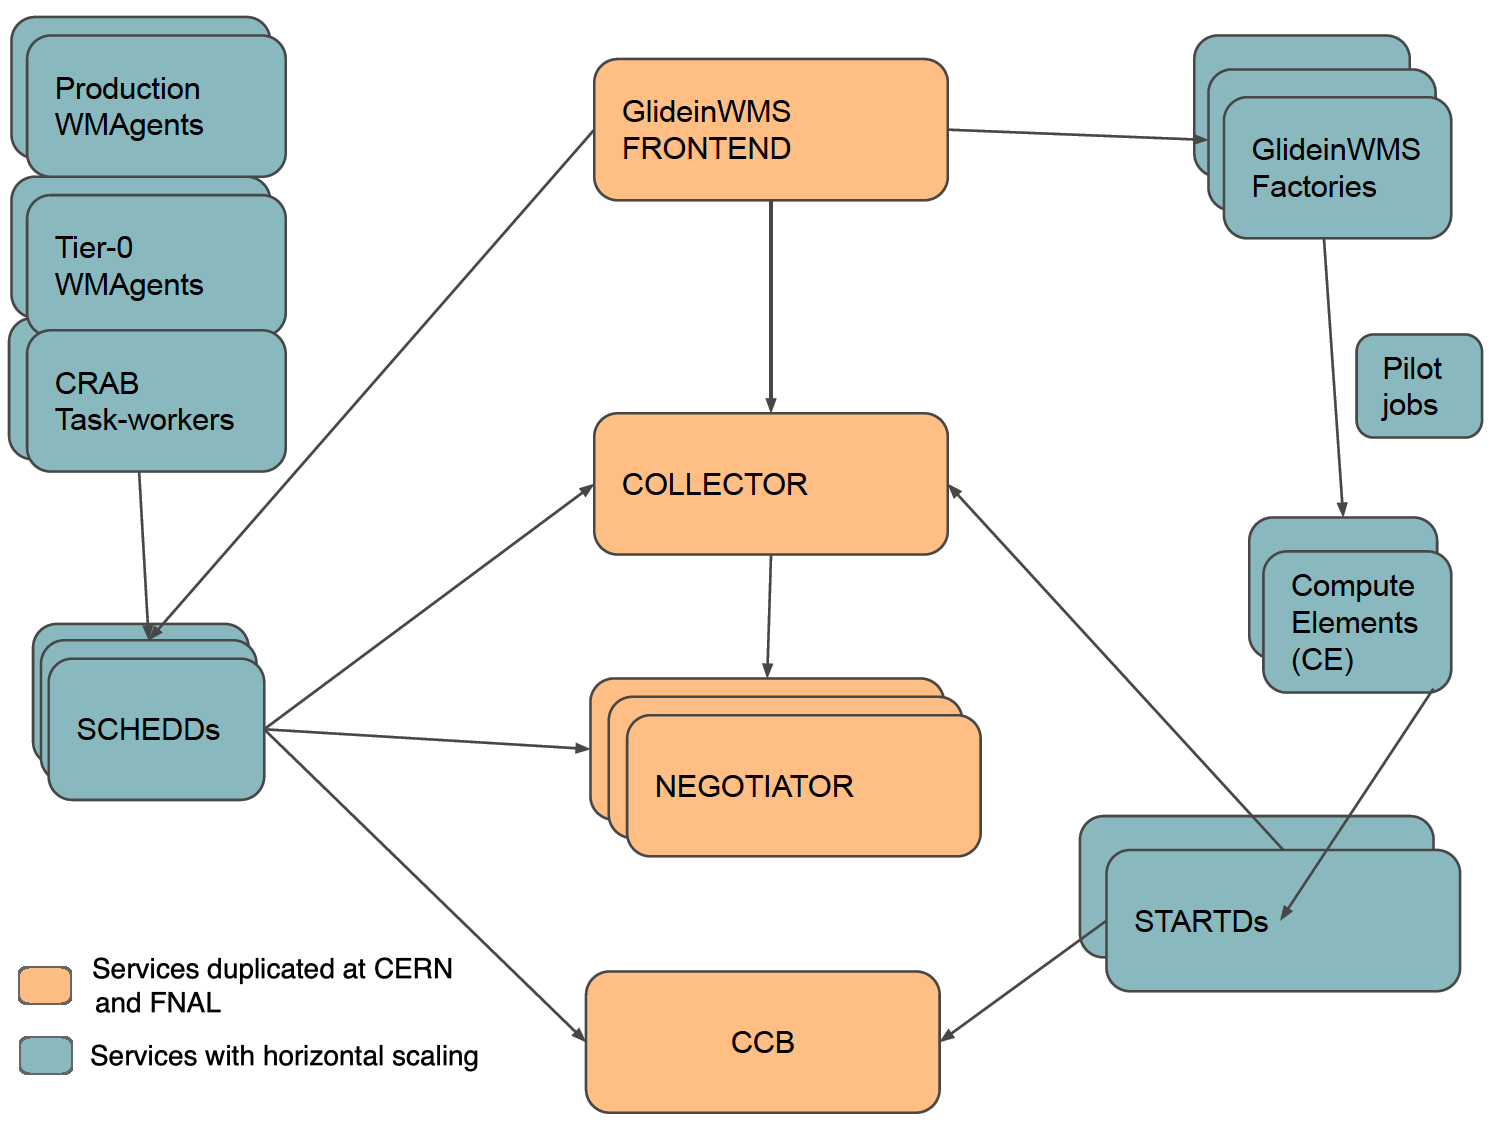
\includegraphics[width=8cm]{figures/SI_HA_and_redundancy.png}
\end{center}
\caption{\label{fig:highavailability}The CMS Global Pool components deployment, as described in section~\ref{sec:deployment}.}
\end{figure}


\section{Scalability}\label{sec:scalability}
The total CPU capacity managed by the SI has been continuously growing in size over the last years (Figure~\ref{fig:scalability}), driven by the increasing resource needs of the collaboration and the progressive incorporation of opportunistic and non-WLCG resources. Operating away from any scalability limiting factor is a critical aspect for our SI, designed to perform in a dynamic environment, adapting to growing resource demands by CMS and resource availability in the WLCG and elsewhere. The SI team proactively detects limitations in the total computing power that our HTCondor pools can harness and use efficiently, regularly running scaling tests~\cite{sicomplexity}~\cite{siscalability} and evolving the SI configuration to operate away from these limits. 

%Front-end and factories capacity to react to oscillating resource demands and provision them. Collector capacity to process the stream of slot updates and keep resource status fresh. Negotiator matchmaking cycle time under control. Total number of workflows we can manage and jobs we can run simultaneously with our pool of schedds

\begin{figure}
\begin{center}
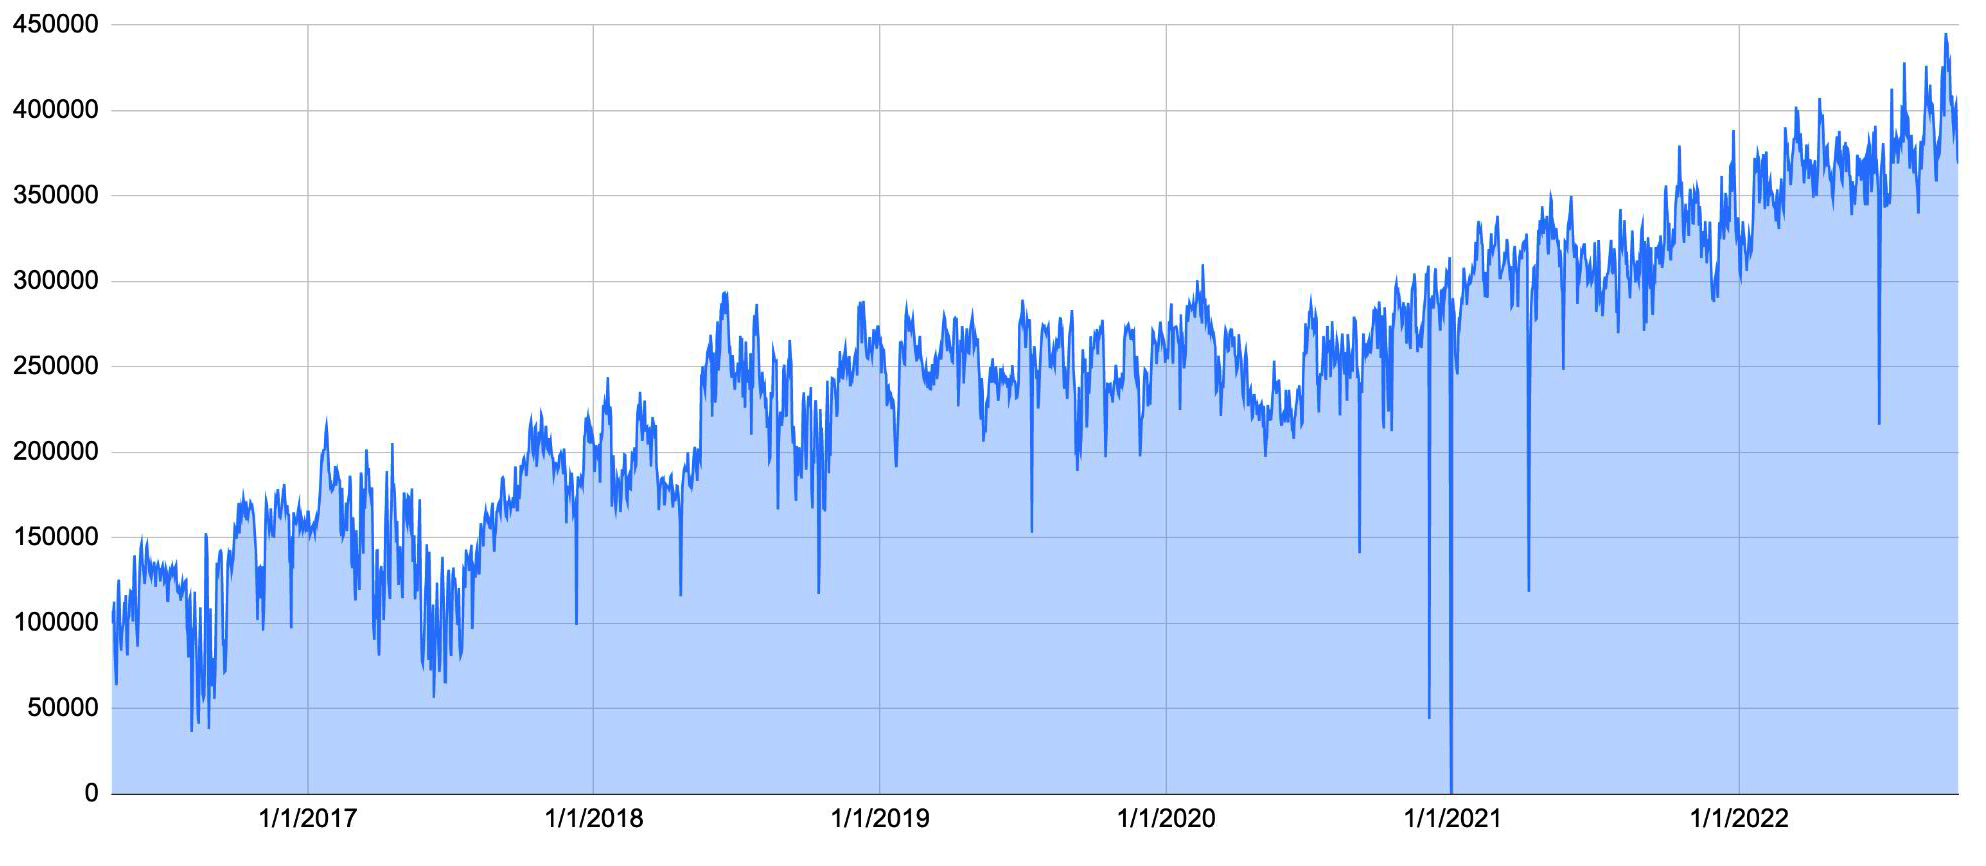
\includegraphics[width=10cm]{figures/CMS_SI_6years.png}
\end{center}
\caption{\label{fig:scalability}Daily average number of CPU cores allocated to CMS over the past years.}
\end{figure}

\section{CMS Tier-0 operations at the start of the LHC Run 3}\label{sec:run3t0}
Since early 2022, in anticipation of the start of the LHC Run 3, the SI was providing resources for Tier-0 commissioning tasks. Given their mission-critical for the CMS collaboration, successive functionality and scalability tests were performed in the first months of 2022 to ensure a smooth restart of data taking operations. In these tests, Tier-0 workloads were injected in bursts to ensure that CPU allocation to these tasks was achieved in sufficient quantity and with the required responsiveness in order to not generate a delay in the completion of e.g. prompt data reconstruction jobs. After July 5th, with the start of stable beam operations at high energy collisions, the SI continued providing CPU to the Tier-0 successfully until the end of data taking period in December as Figure~\ref{fig:tier0} shows.

\begin{figure}
\begin{center}
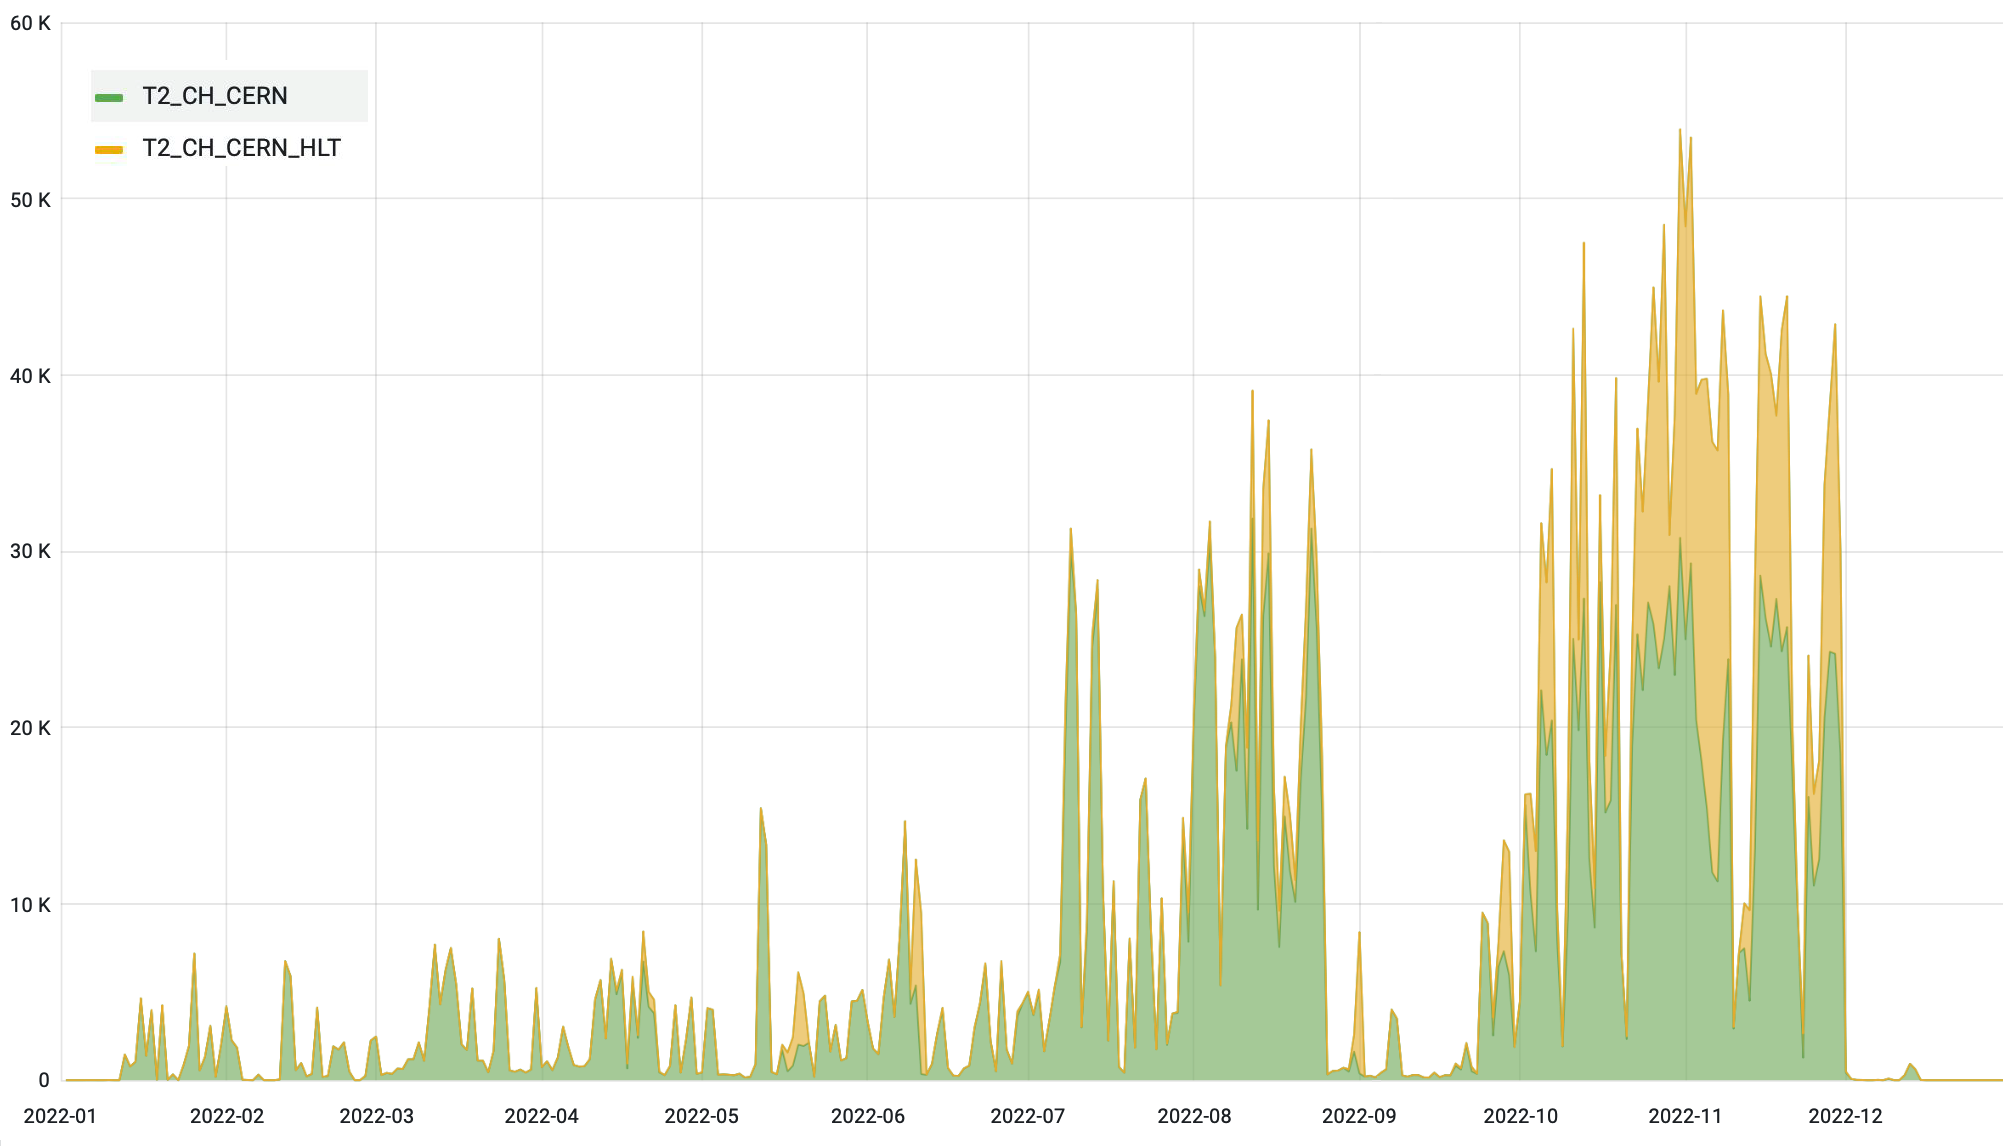
\includegraphics[width=10cm]{figures/Tier0_jobs_CERN_HLT_2022_2.png}
\end{center}
\caption{\label{fig:tier0}Daily average number of CPU cores in use at CERN by CMS Tier-0 tasks during 2022, first year of the LHC Run 3. Resources shown include CPU deployed at the main data center (T2\_CH\_CERN), as well as the cluster formerly dedicated to the CMS high level trigger (HLT) tasks during Run 2 years, currently repurposed as a general resource for CMS computing needs  (T2\_CH\_CERN\_HLT).}
\end{figure}

\section{The Submission Infrastructure 2022 stability tests}\label{sec:drills}
Before the start of the LHC Run 3, the SI team performed a series of exercises to examine the effectiveness of the safety mechanisms embedded in the SI design. In these exercises, carried out in May and June 2022, critical services associated with both the Global and CERN pool infrastructures were intentionally disabled, under close supervision of the SI team, in order to force and observe secondary services reaction. These actions, in the majority of cases, demonstrated the stability of the SI, as they had no impact on the overall performance of the infrastructure. However, some minor effects were detected, then followed by corrective actions. Some of the tests that contributed to improvements of the SI configuration included:

\begin{itemize}
\item Primary HTCondor collector and negotiator processes stopped for for the CERN pool: secondary HTCondor services automatically started running the pool from FNAL. The loss of primary collector did not affect the performance of the primary CERN FE, as it is configured to retrieve pool information from query both collectors (primary and secondary) at once. All job scheduler and execution nodes remained connected to the pool via the backup collector at FNAL. However, a service interruption was detected in our SI monitoring due to an exception triggered when it tried to connect first to the primary collector. The code was corrected and the infrastructure monitoring service recovered.

\item Backup services for the CERN pool disabled: the pool performance, driven by primary services, was not affected. The only minor observed effect was again an interruption of the monitoring service, configured to mainly query the secondary collector, in order to minimize load in the primary one. An alarm was introduced to alert the SI team from the loss of secondary collector.

\item Global Pool primary FE service stopped: the backup FE at FNAL started interacting with the pilot factories. However, the secondary FE requests for resources was being overestimated, as the secondary FE was incorrectly querying both primary and secondary collectors in parallel, leading to some workload double-counting. The backup FE configuration was corrected.
\end{itemize}

\section{Conclusions and future work}\label{sec:conclusions}
As described in this report, the CMS SI has been designed and configured to avoid single points of failure. Considering the critical role of the SI in the capability of the CMS experiment's to take and process collisions data, providing compute resources to the Tier-0 tasks, a number of the tests were performed in order to verify its resilience and stability, before the start of the LHC Run 3 in July 2022. This activity demonstrated that the SI system is stable and fault tolerant in the context of anyone of the central components accidentally becoming unavailable. Some corrections were introduced as a consequence of the tests, mainly in relation to the SI monitoring service.

However, a number of secondary sources of potential instability remain and should also eventually be tested. For example, an outage of the GIT repositories storing the configuration information for each of our services may cause delays in the deployment of new nodes to counter the loss of any main pool element (for example, additional pilot factories or schedds, in case a substantial fraction of them becoming unavailable). In addition, several services (e.g. schedds) are hosted by VMs whose configuration is located in separated CEPH disk volumes, which would be affected in case of file system outages, although the main pool services, running on physical nodes, would not be affected by such an event.

Finally, a key element to the success of the SI operating stably while reaching ever higher scales, has been CMS’s close coordination with the HTCondor and GlideinWMS developers, allowing us to anticipate and remedy future scaling and stability problems. The LHC program extends well into the future, thus the SI is expected to grow in scale as required by CMS needs, while also having to manage an evolving resource landscape. The SI team is committed to maintaining the stability and efficiency of use of the compute capacity available to CMS by continuously evolving our infrastructure adapting it to tools and technology changes.

\ack
This work was partially supported by the Spanish Ministry of Science and Innovation under grants PID2019-110942RB-C21, PID2019-110942RB-C22 and PID2020-113807RA-I00, which include FEDER funds from the European Union, and by the US National Science Foundation under Grant No. 2121686

\section*{References}
\begin{thebibliography}{9}
\bibitem{cms} CMS Collaboration, The CMS experiment at the CERN LHC, 
JINST 3 (2008) S08004, doi:10.1088/1748-0221/3/08/S08004.
\bibitem{wlcg} The Worldwide LHC Computing Grid \url{http://wlcg.web.cern.ch}, accessed March, 2023.
\bibitem{htcondor} The HTCondor Software Suite public web site, \url{https://research.cs.wisc.edu/htcondor/index.html}, accessed March, 2023.
\bibitem{gwms} The Glidein-based Workflow Management System, \url{https://glideinwms.fnal.gov/doc.prd/index.html}, accessed March, 2023.
\bibitem{lhcathome} LHC at Home, \url{https://lhcathome.cern.ch/}, accessed March, 2023. 
%\bibitem{global_pool} J. Balcas et al. ``Using the glideinWMS System as a Common Resource Provisioning Layer in CMS'', J. Phys.: Conf. Ser. \textbf{664} 062031 (2015).
\bibitem{sicomplexity} A. Perez-Calero Yzquierdo et al. ``Evolution of the CMS Global Submission Infrastructure for the HL-LHC Era", EPJ Web Conf. 245 (2020) 03016.
\bibitem{siscalability} A. Perez-Calero Yzquierdo et al. ``Reaching new peaks for the future of the CMS HTCondor Global Pool", EPJ Web Conf. 251 (2021) 02055.
\end{thebibliography}

\end{document}
